\documentclass{article}
\usepackage[utf8]{inputenc}
\usepackage{amssymb}
\usepackage{graphicx}
\usepackage{setspace}
\usepackage{listings}
\usepackage{float}
\usepackage{xcolor}
\usepackage{amsmath}
\usepackage{pgfplots}
\usepackage{enumitem}
\usepackage{subcaption}
\usepackage{hyperref}

\title{\textbf{High Performance Computer Architectures Practical Course \\ - Exercise 4 -} \\[10mm]}
\author{Tutorium 1 \\[10mm] David Jordan (6260776) \\[1mm] Florian Rüffer (7454628) \\[1mm] Michael Samjatin (7485765) \\[10mm]}


\lstset{
    language=C++,
    basicstyle=\ttfamily,
    keywordstyle=\color{blue},
    stringstyle=\color{red},
    commentstyle=\color{green},
    numbers=left,
    numberstyle=\normalsize,
    breaklines=true,
    showstringspaces=false,
    frame=single,
    linewidth=1\linewidth,
    captionpos=b
}
\renewcommand{\lstlistingname}{File}% Listing -> Algorithm
\renewcommand{\lstlistlistingname}{List of \lstlistingname s}% List of Listings -> List of Algorithms

\begin{document}
\maketitle
\newpage
\section{Matrix}
In this task we had to use the Vc implementation to compute the element-wise square root of the matrix. We iterate over the elements of the matrix using nested loops. The outermost loop (variable k) controls the number of iterations (NIter). The second loop (variable l) iterates over the rows of the matrix, and the innermost loop (variable m) iterates over the columns of the matrix.

Within the innermost loop, the scalar float elements of the a and c?\_simdVc arrays are converted to Vc float vector type (float\_v) using the reinterpret\_cast operation. The function f is then applied to the Vc float vector (aVec) using element-wise operations, and the result is stored in the Vc float vector cVec.
Here is a part of the modified Matrix.cpp file: 

\begin{lstlisting}[caption=Matrix.cpp]
   /// Vc
  TStopwatch timerVc; 
  // Iterate NIter times
  for (int k = 0; k < NIter; k++){
    // Iterate over all rows of the matrix
    for(int l = 0; l < N; l++){
      // Itertae over all columns of the matrix
      for(int m = 0; m < N; m+= float_v::Size) {
        // Using reinterpret_cast we convert scalar float array elements to  Vc float vector type
        float_v &aVec = (reinterpret_cast<float_v&>(a[l][m]));
        // Using reinterpret_cast we convert c_simdVc array elements to  Vc float vector type
        float_v &cVec = (reinterpret_cast<float_v&>(c_simdVc[l][m]));
        // Applying the square root template function to the Vc float  vector and storing it in cVec
        cVec = f(aVec);
\end{lstlisting} \\

The resulting output shows a marked speed up of 4.89 resulting from the use of the Vc implementation.

\begin{figure}[H]
    \centering
    \includegraphics[scale=0.3]{matrix_vc_output.png} 
    \caption{Output}
    \label{fig:example}
  \end{figure}
  

\section{Quadratic Equation}
In this exercise we had to complete code solving a set of quadratic equations using both scalar operations and SIMD operations using the Vc library. In the scalar calculations section, a loop iterates over a set of quadratic equations, and for each equation, the code calculates the discriminant and the root using the quadratic formula. In the SIMD  sections, there are two loops, one using Vc and operating on vectors of 'a', 'b', and 'c' coefficients. It copies the coefficients from the input data structure, performs the calculations using Vc vectors, and then copies the roots back to the input data structure.
The second loop also utilizes Vc, but instead of copying the coefficients, it reinterprets the memory of the input data structure as Vc vectors directly. This avoids the need for explicit copying and improves performance. The calculations are performed using the SIMD operations, and the roots are stored back in the input data structure. Here is part of the modified code:  

\begin{lstlisting}[caption=QuadraticEquation.cpp]
 // SIMD calculations with Vc using dataSIMD3 as input (use cast here)
  TStopwatch timerSIMD3;
  for (int io = 0; io < NIterOut; io++)
    for (int i = 0; i < NVectors; i++)
    {
      // Using reinterpret_cast we reinterpret the memory representation of the input data-structure as Vc vectors
      float_v &aV = *(reinterpret_cast<float_v *>(dataSIMD3.data[i].a));
      float_v &bV = *(reinterpret_cast<float_v *>(dataSIMD3.data[i].b));
      float_v &cV = *(reinterpret_cast<float_v *>(dataSIMD3.data[i].c));
      float_v &xV = *(reinterpret_cast<float_v *>(dataSIMD3.data[i].x));

      // We calculate the discriminant and roots here using SIMD operations
      const float_v det = bV * bV - 4 * aV * cV;
      xV = (-bV + sqrt(det)) / (2 * aV);
    }
  timerSIMD3.Stop();
\end{lstlisting} \\

The resulting output reveals that there is a sizeable speedup compared to the scalar calculations,  demonstrating the effectiveness of the use of SIMD operations and the Vc library to efficiently solve multiple quadratic equations in parallel, taking advantage of vectorized instructions for improved performance.

\begin{figure}[H]
    \centering
    \includegraphics[scale=0.3]{qe_out.png} 
    \caption{Output}
    \label{fig:example}
  \end{figure}


\section{Newton}
In this task we have to vectorize the Newton method. As mentioned in the task description
the Newton Method is an interative process to approximate the x-axis intersection. \\[5mm]

\begin{lstlisting}[caption=Newton.cpp]
    float_v FindRootVector(const float_v& p1, const float_v& p2)
    {
      float_v x = 1.f, x_new = 0.f;
      float_m mask(true);
      for( ; !mask.isEmpty(); ) {
          // for(int i = 0; i < 1000; ++i){ 
        x = x_new;
        x_new(mask) = x - F(x,p1,p2) / Fd(x,p1,p2);
        mask = abs((x_new - x)/x_new) > P;
      }
      return x_new;
    }
\end{lstlisting}

\noindent The main idea of vectorizing the Newton method, is the calculation of multiple roots at once.
This comes along with an issue, because if multiple roots are calculate, then also some of those will
reach the desired precision earlier than others. To solve this problem we will use masks.
The underlying principle of masks is a vector with each value mapped to a boolean.
Each boolean value corresponds to the value of another vector.
Using this methodology we can assign 'false' to a corresponding number, which already has our desired precision and therefore
exclude it from further unneccessary calculations.\\

\noindent The first iteration will start with a mask of only 'true' values, as no value has yet reached the desired precision.
This means every value will be updated accordingly with $x - F (x , p1 , p2 ) / Fd (x , p1 , p2 ) $.
The next iteration will only update those values, which need further refinement ($\rightarrow$ mask value equals 'true') with $mask = abs (( x_new - x ) / x_new ) > P $.

\begin{figure}[H]
    \begin{center}
        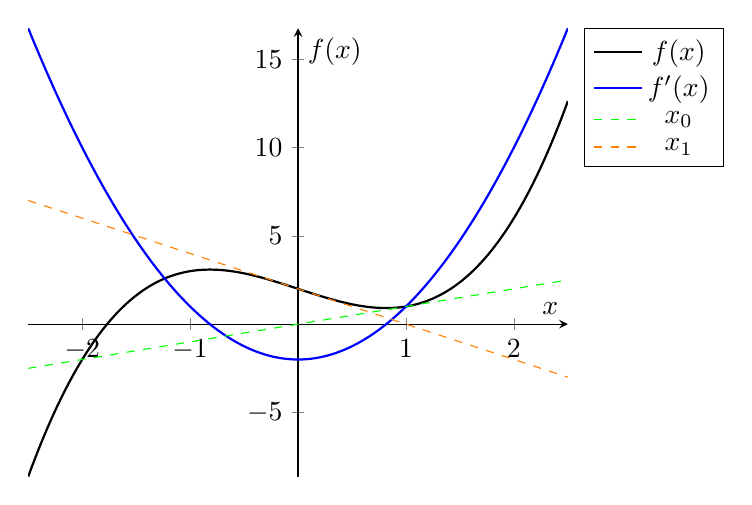
\begin{tikzpicture}[
            declare function={
                func(\x)= \x^3 - 2*\x + 2;
                derivative(\x) = 3*\x^2 - 2;
            }
        ]
        \begin{axis}[
            axis lines=middle,
            xlabel=$x$,
            ylabel={$f(x)$},
            domain=-2.5:2.5,
            samples=200,
            legend pos=outer north east
        ]
        \addplot [thick, black, smooth] {func(x)};
        \addlegendentry{$f(x)$}
        \addplot [thick, blue, smooth] {derivative(x)};
        \addlegendentry{$f'(x)$}
        
        \pgfmathsetmacro{\a}{1}
        \pgfmathsetmacro{\b}{\a - func(\a)/derivative(\a)}
        
        \addplot [green, dashed, samples=2, domain=(-2.5:2.5)] {(func(\a) + derivative(\a) * (x - \a))};
        \addlegendentry{$x_0$}
        
        \pgfmathsetmacro{\a}{\b}
        \pgfmathsetmacro{\b}{\a - func(\a)/derivative(\a)}
        
        \addplot [orange, dashed, samples=2, domain=(-2.5:2.5)] {(func(\a) + derivative(\a) * (x - \a))};
        \addlegendentry{$x_1$}
        
        \pgfmathsetmacro{\a}{\b}
        \pgfmathsetmacro{\b}{\a - func(\a)/derivative(\a)}
        
        \end{axis}
        \end{tikzpicture}
    \end{center}   
\end{figure}
\newpage
\section{Random Access}
The first part of this exercise is done by gathering the data from the input
arry to the tmp float\_v variable according to the index array. This is done
by initializing a uint\_v vector and it's corresponding indexes. If this is
done, the goal of the subtask can be achieved by running the gather function:\\
\begin{lstlisting}[caption=gathering data]
    tmp.gather(input, ind);
\end{lstlisting}
Now we want to filter the data - from the tmp variable every value larger than
0.5. Therefore we create a specific mask with the following code:
float\_m mask = tmp $>$ 0.5f;\\
With this mask, and a new initialized variable, where we want to safe the data,
we can run the "gather" function again, with adapted parameters:\\
\begin{lstlisting}[caption=gathering filtered data]
    tmp2.gather(input, ind, mask);
\end{lstlisting}
The last part of this exercise is to put the data from the tmp float\_v variable
to the ouput array, when it satisfies a given condition.
The condition is, that all values from tmp, that are smaller than 0.5, are 
put to the array "ouput" at the places given by indices.\\
We could create a new mask, but because this mask's type is identical to
the mask above (and because the solutions does it like this), we reuse the mask
(of course with adjusted filter $<$ 0.5).\\
Lastly one can just use the scatter function with the added parameters to get the
wished results to the tmp variable.
\begin{lstlisting}[caption=scattering]
    tmp.scatter(input, ind, mask);
\end{lstlisting}






\end{document}
